\hypertarget{_s_c_p_i__specific_regs_8h}{\section{scpi/\-S\-C\-P\-I\-\_\-specific\-Regs.h File Reference}
\label{_s_c_p_i__specific_regs_8h}\index{scpi/\-S\-C\-P\-I\-\_\-specific\-Regs.\-h@{scpi/\-S\-C\-P\-I\-\_\-specific\-Regs.\-h}}
}
This graph shows which files directly or indirectly include this file\-:\nopagebreak
\begin{figure}[H]
\begin{center}
\leavevmode
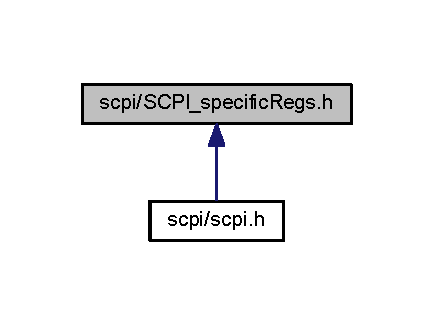
\includegraphics[width=208pt]{_s_c_p_i__specific_regs_8h__dep__incl}
\end{center}
\end{figure}


\subsection{Detailed Description}
This file creates the application specific questionable status registers and provides the functions for managing them

These registers and their bits can be changed by by the user to suit the application in use, though they should follow the guidelines and conventions laid out in I\-E\-E\-E 488.\-2-\/1992 and S\-C\-P\-I-\/1999

Please follow the information in the parser documentation and the file S\-C\-P\-I\-\_\-specific\-Regs.\-c on how to add or change questionable event status registers 